\chapter{Resultados}\label{cap:resultados}

En este capítulo se presentan los resultados de la evaluación experimental. Primero se muestra el desempeño de los ocho SLM al clasificar lotes de 50 eventos frente al \textit{ground truth}, después con lotes de 30 y de 20 eventos, y la consistencia de cada modelo al reducir el tamaño de lote. A continuación se compara Qwen3.5-9B antes y después del ajuste fino, y por último se presentan los resultados de la simulación en flujo continuo, en la que el \textit{pipeline} completo analizó un flujo de logs con errores inyectados. En todas las comparaciones, la significancia se determinó con pruebas de permutación pareadas y corrección de Holm; los intervalos de confianza del 95\,\% de las métricas se calcularon con \textit{bootstrap} por bloques, y los de la tasa de detección de la simulación, con el intervalo de Wilson.

\section{Detección de errores con lotes de 50 eventos}\label{sec:res_n50}

La primera evaluación comparó la respuesta de cada SLM sobre los 4\,463 lotes de 50 eventos con la etiqueta del \textit{ground truth}, que contiene 130 lotes con error. Los lotes en que un modelo no dio una respuesta válida se contaron como fallos de ese modelo, de modo que todos se calificaron sobre los mismos 4\,463 lotes. En la tabla~\ref{tab:res_n50} se presentan las métricas, ordenadas por MCC. Como referencia para leerlas, un clasificador al azar, que marca los lotes como error sin considerar su contenido, obtiene en promedio un MCC de 0, una \textit{balanced accuracy} y un AUC de 0.5, y una AP igual a la proporción de lotes con error, que aquí es 0.029. Un modelo cuyos valores se acercan a esos no distingue los lotes con error de los normales, y cuanto más se acercan a 1, mejor los distingue.

\begin{table}[H]
\centering
\caption{Métricas de los SLM con $N = 50$ frente al \textit{ground truth} (4\,463 lotes, 130 con error). Bal. acc.: \textit{balanced accuracy}; FA: falsas alarmas; EO: errores omitidos.}
\label{tab:res_n50}\label{tab:res_n50_final}
\footnotesize
\setlength{\tabcolsep}{4pt}
\begin{tabular}{@{}lrrrrrrrrr@{}}
\toprule
\textbf{Modelo} & \textbf{Precisión} & \textbf{Recall} & \textbf{$F_1$} & \textbf{MCC} & \textbf{Bal. acc.} & \textbf{AUC} & \textbf{AP} & \textbf{FA} & \textbf{EO} \\
\midrule
Qwen3.5-9B & 0.174 & 0.962 & 0.295 & 0.377 & 0.912 & 0.987 & 0.878 & 593 & 5 \\
Granite-4.1-3B & 0.099 & 0.962 & 0.179 & 0.260 & 0.849 & 0.932 & 0.395 & 1\,142 & 5 \\
Phi-3.5-mini & 0.097 & 0.862 & 0.174 & 0.238 & 0.810 & 0.897 & 0.178 & 1\,046 & 18 \\
Gemma-3-4B & 0.046 & 0.954 & 0.089 & 0.126 & 0.683 & 0.833 & 0.129 & 2\,548 & 6 \\
Ling-3.0-tiny & 0.040 & 0.962 & 0.076 & 0.097 & 0.631 & 0.933 & 0.491 & 3\,034 & 5 \\
Ministral-3-3B & 0.033 & 0.985 & 0.064 & 0.059 & 0.559 & 0.877 & 0.353 & 3\,757 & 2 \\
Llama-3.2-1B \textit{log-analyzer} & 0.079 & 0.092 & 0.085 & 0.056 & 0.530 & 0.549 & 0.069 & 140 & 118 \\
SmolLM2-1.7B-Instruct & 0.049 & 0.092 & 0.064 & 0.028 & 0.519 & 0.430 & 0.031 & 234 & 118 \\
\bottomrule
\end{tabular}
\normalsize
\end{table}

La tabla muestra dos comportamientos opuestos. Los seis primeros modelos detectan casi todos los errores, pero emiten muchas falsas alarmas, ya que marcan como error una parte grande de los lotes que el \textit{ground truth} considera normales. Los dos modelos más pequeños hacen lo contrario: casi no emiten alertas y omiten la mayoría de los errores, y aun así obtienen la mayor especificidad (0.968 y 0.946) y la mayor exactitud (0.942 y 0.921) de los ocho modelos. Con un 2.9\,\% de lotes con error, esa exactitud solo refleja que casi no emiten alertas, y por eso la tabla se ordena por MCC.

Las columnas de MCC y de AP miden aspectos distintos: el MCC evalúa la respuesta sí o no del modelo, y la AP, el orden en que su probabilidad de error coloca los lotes. Por eso un modelo puede quedar abajo en MCC y arriba en AP, como ocurre con Ling-3.0-tiny y Ministral-3-3B: su probabilidad separa bien los lotes con error de los normales, pero su respuesta marca como error casi todos los lotes. En la figura~\ref{fig:res_pr_n50} se comparan el valor de AP y su MCC correspondiente.

\figpendiente{fig:res_pr_n50}{Curvas de precisión-\textit{recall} de los ocho SLM con $N = 50$ frente al \textit{ground truth}.}{Curvas de precisión-\textit{recall} superpuestas de los ocho modelos, con la AP de cada uno en la leyenda y la línea del clasificador al azar (0.029). Ya existe una versión: \texttt{pr\_comparison\_knn\_\_n50.png} (carpeta \texttt{summary\_plots} de \texttt{analysis/batch\_size\_matrix}).}

La prueba global rechazó la igualdad de los ocho modelos en las ocho métricas, con un valor $p$ ajustado menor que 0.001, lo que indica que en cada métrica al menos un modelo difiere de los demás. Las comparaciones por pares muestran, sin embargo, que no todos los modelos se distinguen entre sí. El \textit{recall} es la métrica con menos diferencias: 14 de los 28 pares no fueron significativos, y Qwen3.5-9B no se distinguió en ella de Granite-4.1-3B, Gemma-3-4B, Ling-3.0-tiny ni Ministral-3-3B, con un valor $p$ ajustado de 1.0, ni de Phi-3.5-mini, con 0.057. En precisión, $F_1$, MCC y \textit{balanced accuracy}, los pares no significativos se concentraron entre los modelos de menor desempeño, y Granite-4.1-3B y Phi-3.5-mini tampoco se distinguieron en precisión, $F_1$ ni MCC. En AUC solo dos pares no fueron significativos, Ling-3.0-tiny frente a Granite-4.1-3B y Ministral-3-3B frente a Phi-3.5-mini, y en exactitud y especificidad todos lo fueron. Qwen3.5-9B, en cambio, superó a cada uno de los otros siete modelos en precisión, $F_1$, MCC, \textit{balanced accuracy} y AUC, con un valor $p$ ajustado de 0.003, y el intervalo de confianza del 95\,\% de su MCC fue de 0.31 a 0.43.

\subsection{Respuestas inválidas y tiempo de ejecución}

Cuatro modelos dejaron lotes sin respuesta válida: Phi-3.5-mini, 2; Gemma-3-4B, 8; Ling-3.0-tiny, 3; y SmolLM2-1.7B-Instruct, 128. Si esos lotes se excluyen en lugar de contarse como fallos, el orden de la tabla~\ref{tab:res_n50} no cambia, y solo SmolLM2-1.7B-Instruct varía de forma apreciable, de un MCC de 0.028 a 0.073 y de un AUC de 0.430 a 0.580, porque sus lotes fallidos contienen 30 de los 130 errores.

El tiempo de cada ejecución completa con $N = 50$ se muestra en la tabla~\ref{tab:res_tiempos}. Los tiempos corresponden al reloj de cada ejecución y dependen del equipo y del motor de inferencia, por lo que no miden solo al modelo. \falta{confirmar en qué equipo corrió cada modelo con $N = 50$: se asumió el Equipo 1 para todos salvo SmolLM2, según la tabla de equipos}

\begin{table}[H]
\centering
\caption{Tiempo de clasificación de los 4\,463 lotes con $N = 50$. El equipo corresponde a la tabla~\ref{tab:met_equipos}.}
\label{tab:res_tiempos}
\small
\begin{tabular}{@{}lllrr@{}}
\toprule
\textbf{Modelo} & \textbf{Equipo} & \textbf{Motor} & \textbf{Tiempo total (h)} & \textbf{s por lote} \\
\midrule
Granite-4.1-3B & Equipo 1 & Transformers & 1.79 & 1.44 \\
Llama-3.2-1B \textit{log-analyzer} & Equipo 1 & Ollama & 2.37 & 1.91 \\
SmolLM2-1.7B-Instruct & Equipo 2 & Transformers & 2.84 & 2.29 \\
Qwen3.5-9B & Equipo 1 & Ollama & 2.96 & 2.38 \\
Ling-3.0-tiny & Equipo 1 & Ollama & 3.08 & 2.49 \\
Ministral-3-3B & Equipo 1 & Ollama & 3.90 & 3.14 \\
Phi-3.5-mini & Equipo 1 & Transformers & 3.92 & 3.16 \\
Gemma-3-4B & Equipo 1 & Transformers & 6.29 & 5.07 \\
\bottomrule
\end{tabular}
\normalsize
\end{table}
% Tiempos: totals.elapsed_seconds de cada run_*.json en analysis/batch_size_matrix/n50/. El equipo se tomó de la tabla de equipos (Equipo 2: SmolLM2 con N=50); confirmar que el resto corrió en el Equipo 1.

\section{Detección de errores con lotes de 30 y de 20 eventos}\label{sec:res_n30_n20}

Con lotes de 30 y de 20 eventos, cada lote recibió la etiqueta del lote de 50 del \textit{ground truth} con el texto más parecido. Como control, con $N = 50$ el vecino de cada lote fue siempre el mismo lote y la evaluación reprodujo exactamente las métricas de la tabla~\ref{tab:res_n50}, y con lotes pequeños la etiqueta prestada coincidió en el 97.7\,\% de los lotes con la del lote de 50 que contiene los mismos eventos. La similitud del coseno con el vecino tuvo una mediana de 0.959 con $N = 30$ y de 0.947 con $N = 20$, pero fue menor en los lotes cuya referencia es un error, por lo que la etiqueta prestada es menos segura justo en esos lotes. Por eso las cifras de cada tamaño sirven para comparar los modelos entre sí, pero no para compararlas con las de $N = 50$. En la tabla~\ref{tab:res_n30_n20} se presentan las métricas principales con ambos tamaños.

\begin{table}[H]
\centering
\caption{Métricas de los SLM con $N = 30$ (7\,437 lotes, 176 con error) y $N = 20$ (11\,156 lotes, 227 con error) frente a la etiqueta del lote de 50 más parecido. Prec.: precisión; Bal. acc.: \textit{balanced accuracy}. AP al azar: 0.024 y 0.020.}
\label{tab:res_n30_n20}
\footnotesize
\setlength{\tabcolsep}{3pt}
\begin{tabular}{@{}lrrrrrrrrrr@{}}
\toprule
 & \multicolumn{5}{c}{\textbf{$N = 30$}} & \multicolumn{5}{c}{\textbf{$N = 20$}} \\
\cmidrule(lr){2-6}\cmidrule(l){7-11}
\textbf{Modelo} & \textbf{Prec.} & \textbf{Recall} & \textbf{MCC} & \textbf{Bal. acc.} & \textbf{AP} & \textbf{Prec.} & \textbf{Recall} & \textbf{MCC} & \textbf{Bal. acc.} & \textbf{AP} \\
\midrule
Qwen3.5-9B & 0.159 & 0.761 & 0.318 & 0.832 & 0.569 & 0.164 & 0.678 & 0.308 & 0.803 & 0.520 \\
Granite-4.1-3B & 0.099 & 0.824 & 0.246 & 0.821 & 0.181 & 0.111 & 0.767 & 0.259 & 0.819 & 0.257 \\
Phi-3.5-mini & 0.123 & 0.625 & 0.242 & 0.759 & 0.141 & 0.111 & 0.586 & 0.223 & 0.744 & 0.139 \\
Gemma-3-4B & 0.063 & 0.875 & 0.182 & 0.780 & 0.158 & 0.093 & 0.837 & 0.244 & 0.834 & 0.201 \\
SmolLM2-1.7B-Instruct & 0.081 & 0.153 & 0.081 & 0.555 & 0.061 & 0.138 & 0.163 & 0.131 & 0.571 & 0.119 \\
Ling-3.0-tiny & 0.031 & 0.852 & 0.064 & 0.600 & 0.371 & 0.028 & 0.846 & 0.066 & 0.613 & 0.321 \\
Ministral-3-3B & 0.028 & 0.960 & 0.056 & 0.571 & 0.188 & 0.026 & 0.996 & 0.074 & 0.607 & 0.179 \\
Llama-3.2-1B \textit{log-analyzer} & 0.051 & 0.125 & 0.045 & 0.534 & 0.067 & 0.027 & 0.366 & 0.029 & 0.546 & 0.077 \\
\bottomrule
\end{tabular}
\normalsize
\end{table}

La tabla se lee igual que la de $N = 50$ y muestra los mismos dos grupos: los modelos más capaces detectan la mayoría de los errores con poca precisión, y los más pequeños marcan pocos lotes. Los modelos difirieron en las ocho métricas con ambos tamaños, con un valor $p$ ajustado menor que 0.001 en la prueba global. Qwen3.5-9B obtuvo el mayor MCC y la mayor AP con ambos tamaños; el intervalo del 95\,\% de su MCC fue de 0.26 a 0.37 con $N = 30$ y de 0.25 a 0.36 con $N = 20$, y superó en MCC a cada uno de los demás modelos con un valor $p$ ajustado de 0.003, salvo frente a Granite-4.1-3B con $N = 20$, donde fue de 0.010. Solo SmolLM2-1.7B-Instruct dejó lotes sin respuesta válida, 16 con $N = 30$ y 4 con $N = 20$, y contarlos como fallos cambió 7 de las 224 comparaciones por pares con $N = 30$ y 2 con $N = 20$, ninguna de Qwen3.5-9B en precisión, $F_1$ o MCC.

\section{Consistencia al reducir el tamaño de lote}\label{sec:res_consistencia}

Las cifras de la sección anterior no indican si un modelo clasifica igual con menos contexto, porque cada tamaño se compara con una referencia distinta. Para medirlo, cada lote de 30 o de 20 eventos se comparó con la respuesta que el mismo modelo dio con $N = 50$ al lote de texto más parecido. Ese vecino fue el lote de 50 del que proviene el lote pequeño solo en el 8\,\% de los lotes con $N = 30$ y en el 5\,\% con $N = 20$; en el resto, fue un lote de contenido parecido de otra parte del corpus. En las tablas de esta sección, el kappa indica cuánto coincide cada modelo consigo mismo por encima de lo esperado por azar, y las dos últimas columnas muestran de qué lado está el desacuerdo: la proporción de repetidas baja cuando el modelo deja de marcar con el lote pequeño lo que marcaba con 50 eventos, y la de coincidentes, cuando marca lotes que con 50 eventos consideraba normales. En la tabla~\ref{tab:res_consistencia} se presentan los resultados con $N = 30$.

\begin{table}[H]
\centering
\caption{Consistencia de cada modelo con $N = 30$ frente a sus propias respuestas con $N = 50$ (7\,437 lotes). Alertas: lotes marcados como error; Repetidas: proporción de alertas de $N = 50$ que el modelo repite con el lote pequeño; Coincidentes: proporción de alertas del lote pequeño cuya referencia también era una alerta.}
\label{tab:res_consistencia}
\small
\setlength{\tabcolsep}{4pt}
\begin{tabular}{@{}lrrrcrr@{}}
\toprule
 & \multicolumn{2}{c}{\textbf{Alertas}} & & & & \\
\cmidrule(lr){2-3}
\textbf{Modelo} & \textbf{$N = 50$} & \textbf{$N = 30$} & \textbf{Kappa} & \textbf{IC 95\,\%} & \textbf{Repetidas} & \textbf{Coincidentes} \\
\midrule
Granite-4.1-3B & 1\,631 & 1\,464 & 0.82 & [0.80, 0.84] & 0.81 & 0.91 \\
Phi-3.5-mini & 1\,477 & 893 & 0.60 & [0.57, 0.62] & 0.53 & 0.87 \\
Qwen3.5-9B & 896 & 845 & 0.46 & [0.42, 0.50] & 0.51 & 0.54 \\
Gemma-3-4B & 4\,449 & 2\,432 & 0.27 & [0.24, 0.30] & 0.45 & 0.82 \\
SmolLM2-1.7B-Instruct & 415 & 305 & 0.23 & [0.19, 0.28] & 0.23 & 0.32 \\
Ling-3.0-tiny & 5\,410 & 4\,883 & 0.06 & [0.04, 0.08] & 0.67 & 0.75 \\
Ministral-3-3B & 6\,748 & 6\,110 & 0.05 & [0.03, 0.08] & 0.83 & 0.92 \\
Llama-3.2-1B \textit{log-analyzer} & 129 & 429 & 0.03 & [0.00, 0.06] & 0.12 & 0.04 \\
\bottomrule
\end{tabular}
\normalsize
\end{table}

Con $N = 30$, el acuerdo superó al azar en todos los modelos, con un valor $p$ ajustado menor que 0.001, salvo el Llama-3.2-1B \textit{log-analyzer}, que lo superó con 0.007. En Ling-3.0-tiny, Ministral-3-3B y el Llama-3.2-1B \textit{log-analyzer}, sin embargo, esa significancia se debe más al gran número de lotes que a un acuerdo real, y su proporción alta de repetidas proviene de marcar casi todo como error. Los modelos difirieron entre sí en las cuatro métricas de consistencia, con un valor $p$ ajustado menor que 0.001, y 24 de las 28 comparaciones por pares del kappa fueron significativas; no se distinguieron SmolLM2-1.7B-Instruct de Gemma-3-4B, ni Ling-3.0-tiny, Ministral-3-3B y el Llama-3.2-1B \textit{log-analyzer} entre sí. Con 20 eventos por lote, el contexto se reduce aún más, y sus resultados se presentan en la tabla~\ref{tab:res_consistencia_n20}.

\begin{table}[H]
\centering
\caption{Consistencia de cada modelo con $N = 20$ frente a sus propias respuestas con $N = 50$ (11\,156 lotes). Las columnas son las de la tabla~\ref{tab:res_consistencia}.}
\label{tab:res_consistencia_n20}
\small
\setlength{\tabcolsep}{4pt}
\begin{tabular}{@{}lrrrcrr@{}}
\toprule
 & \multicolumn{2}{c}{\textbf{Alertas}} & & & & \\
\cmidrule(lr){2-3}
\textbf{Modelo} & \textbf{$N = 50$} & \textbf{$N = 20$} & \textbf{Kappa} & \textbf{IC 95\,\%} & \textbf{Repetidas} & \textbf{Coincidentes} \\
\midrule
Granite-4.1-3B & 1\,947 & 1\,570 & 0.81 & [0.79, 0.82] & 0.75 & 0.94 \\
Phi-3.5-mini & 1\,915 & 1\,192 & 0.61 & [0.59, 0.63] & 0.54 & 0.86 \\
Qwen3.5-9B & 1\,249 & 940 & 0.46 & [0.43, 0.49] & 0.45 & 0.60 \\
Gemma-3-4B & 4\,415 & 2\,034 & 0.40 & [0.38, 0.42] & 0.40 & 0.87 \\
SmolLM2-1.7B-Instruct & 571 & 252 & 0.11 & [0.08, 0.14] & 0.10 & 0.23 \\
Ling-3.0-tiny & 9\,153 & 6\,970 & 0.04 & [0.02, 0.05] & 0.63 & 0.83 \\
Ministral-3-3B & 10\,557 & 8\,761 & $-$0.04 & [$-$0.05, $-$0.03] & 0.78 & 0.94 \\
Llama-3.2-1B \textit{log-analyzer} & 116 & 3\,073 & 0.00 & [0.00, 0.01] & 0.33 & 0.01 \\
\bottomrule
\end{tabular}
\normalsize
\end{table}

Con $N = 20$, el acuerdo superó al azar en seis modelos, con un valor $p$ ajustado menor que 0.001, pero no en Ministral-3-3B ni en el Llama-3.2-1B \textit{log-analyzer} (valores $p$ de 1.0 y 0.24), cuyas respuestas con 20 eventos no guardan relación con las de 50. Los modelos también difirieron en las cuatro métricas, y como las 28 comparaciones por pares del kappa fueron significativas, el orden es estricto: Granite-4.1-3B, Phi-3.5-mini, Qwen3.5-9B, Gemma-3-4B, SmolLM2-1.7B-Instruct, Ling-3.0-tiny, Llama-3.2-1B \textit{log-analyzer} y Ministral-3-3B.

Con ambos tamaños, ningún modelo conservó por completo su clasificación, y se distinguen tres comportamientos. Granite-4.1-3B fue el más consistente: repitió la mayoría de sus alertas, y casi todas sus alertas con lotes pequeños coincidieron con una de $N = 50$. Qwen3.5-9B, el mejor frente al \textit{ground truth}, solo concordó moderadamente consigo mismo: emitió un número parecido de alertas, pero sobre lotes distintos. Phi-3.5-mini y Gemma-3-4B, por su parte, emitieron muchas menos alertas con menos contexto, aunque las que mantuvieron coincidieron en su mayoría con una alerta de $N = 50$. Además, los lotes pequeños multiplican las llamadas al modelo por 1.7 con $N = 30$ y por 2.5 con $N = 20$.

\figpendiente{fig:res_kappa}{Kappa de Cohen de cada modelo con $N = 30$ y $N = 20$ frente a sus respuestas con $N = 50$.}{Gráfico de puntos con barras de error: un renglón por modelo, ordenado por kappa; dos marcadores por modelo ($N = 30$ y $N = 20$) con su intervalo del 95\,\%; línea vertical en kappa = 0 (azar). Datos en \texttt{analysis/significance/self\_consistency\_\_n30} y \texttt{\_\_n20}.}

\section{Efecto del ajuste fino}\label{sec:res_ajuste}

La comparación del modelo Qwen3.5-9B, el cual su evaluación presentó el mejor balance entre falsas alarmas y detección de errores, y su versión ajustada con LoRA, se hizo sobre los 892 lotes de la parte de prueba de la tabla~\ref{tab:met_particion}, de los cuales 29 contienen un error; como esa proporción es del 3.3\,\%, la AP de referencia de un clasificador al azar en esta parte es 0.033, en lugar del 0.029 del corpus completo. En la tabla~\ref{tab:res_ajuste} se presentan los resultados de ambos modelos, con su respuesta directa y con el umbral sobre la probabilidad de error elegido en la validación.

\begin{table}[H]
\centering
\caption{Qwen3.5-9B base y ajustado sobre los 892 lotes de prueba (29 con error). Umbral: umbral sobre la probabilidad de error elegido en la validación (--: respuesta directa del modelo); FA: falsas alarmas; EO: errores omitidos; Bal. acc.: \textit{balanced accuracy}.}
\label{tab:res_ajuste}
\footnotesize
\setlength{\tabcolsep}{4pt}
\begin{tabular}{@{}lcrrrrrrcrr@{}}
\toprule
\textbf{Modelo} & \textbf{Umbral} & \textbf{FA} & \textbf{EO} & \textbf{Precisión} & \textbf{Recall} & \textbf{$F_1$} & \textbf{Bal. acc.} & \textbf{MCC [IC 95\,\%]} & \textbf{AUC} & \textbf{AP} \\
\midrule
Base & -- & 113 & 1 & 0.20 & 0.97 & 0.33 & 0.92 & 0.41 [0.28, 0.51] & 0.990 & 0.916 \\
Base con umbral & 0.959 & 2 & 6 & 0.92 & 0.79 & 0.85 & 0.90 & 0.85 [0.73, 0.93] & 0.990 & 0.916 \\
\textbf{Ajustado} & -- & \textbf{1} & \textbf{2} & \textbf{0.96} & \textbf{0.93} & \textbf{0.95} & \textbf{0.96} & \textbf{0.95 [0.88, 1.00]} & 0.988 & 0.936 \\
Ajustado con umbral & 0.978 & 1 & 4 & 0.96 & 0.86 & 0.91 & 0.93 & 0.91 [0.84, 0.98] & 0.988 & 0.936 \\
\bottomrule
\end{tabular}
\normalsize
\end{table}

La diferencia principal entre ambos modelos está en las falsas alarmas: con el modelo base, cuatro de cada cinco alertas eran falsas, mientras que con el ajustado casi todas correspondieron a errores reales, a cambio de un error omitido más. La prueba global rechazó la igualdad en precisión, $F_1$, exactitud, especificidad y MCC, con un valor $p$ ajustado menor que 0.001, pero no en \textit{recall}, \textit{balanced accuracy} ni AUC. En las comparaciones por pares, el modelo ajustado superó al base en esas cinco métricas, todas con un valor $p$ ajustado menor que 0.001.

El umbral también mejoró de forma significativa al modelo base, con un valor $p$ ajustado menor que 0.001 en MCC. Frente a esa variante, en cambio, la ventaja del ajustado en MCC no fue significativa (valor $p$ ajustado de 0.20), y tampoco la del \textit{recall}; con solo 29 errores, la prueba tiene poca potencia para diferencias de ese tamaño. Aun así, el ajustado omitió menos errores sin necesitar un umbral calibrado, y los dos errores que siguió omitiendo también los omitió el modelo base con umbral. Al modelo ajustado, en cambio, el umbral no le favoreció: perdió dos errores sin ganar precisión.

La AP de ambos modelos es casi igual, y sus curvas de precisión-\textit{recall} prácticamente se superponen, como se observa en la figura~\ref{fig:res_pr_ajuste}. El modelo base ya ordenaba bien los lotes por su probabilidad de error, y lo que cambió con el ajuste fino fue la decisión sí o no.

\figpendiente{fig:res_pr_ajuste}{Curvas de precisión-\textit{recall} de Qwen3.5-9B base y ajustado sobre los lotes de prueba.}{Dos curvas superpuestas (base, AP = 0.916; ajustado, AP = 0.936) con la línea del azar (0.033) y los puntos de operación de las cuatro variantes de la tabla anterior. Ya existe una versión en \texttt{analysis/finetune/test\_split/pr\_curves.png}.}

\section{Simulación en flujo continuo con errores inyectados}\label{sec:res_simulacion}

La simulación pasó del clasificador al sistema completo: el \textit{pipeline} leyó por HTTP un flujo de 4\,549 lotes con 216 incidentes inyectados y los analizó con Qwen3.5-9B base y ajustado, con cada uno de los 18 métodos de caché. Ninguna de las ejecuciones tuvo respuestas inválidas. Los resultados se presentan en cuatro partes: la detección en el flujo completo, la comparación entre ambos modelos en los lotes de prueba, la dependencia del SLM y la latencia.

\subsection{Detección en el flujo completo}

En las tablas~\ref{tab:res_sim_deteccion} y~\ref{tab:res_sim_deteccion_ft} se compara, para cada método de caché y umbral, cuántos incidentes detectó cada modelo, cuántas falsas alarmas emitió y qué parte de los lotes llegó al SLM, en el modo de velocidad máxima. La primera fila, sin caché, es la referencia. La columna de omitidos en caché cuenta los incidentes no detectados cuyo lote respondió la caché sin consultar al SLM; no todos son pérdidas causadas por la caché, porque el SLM solo tampoco detecta algunos de esos lotes, y lo que la caché cuesta en realidad es la diferencia de incidentes detectados respecto de la primera fila. Los intervalos de Wilson del 95\,\% de la detección con el SLM solo fueron de 91.1\,\% a 97.1\,\% con el modelo base y de 88.9\,\% a 95.7\,\% con el ajustado.

\begin{table}[H]
\centering
\caption{Detección en el flujo completo con el modelo base (4\,549 lotes, 216 incidentes), velocidad máxima. Omitidos en caché: incidentes no detectados cuyo lote respondió la caché sin consultar al SLM; FA: falsas alarmas; Bal. acc.: \textit{balanced accuracy}; Uso SLM: lotes enviados al modelo.}
\label{tab:res_sim_deteccion}
\footnotesize
\setlength{\tabcolsep}{3pt}
\begin{tabular}{@{}llrrrrrrrr@{}}
\toprule
\textbf{Método} & \textbf{Umbral} & \textbf{Detectados} & \textbf{\begin{tabular}[b]{@{}c@{}}Omitidos\\en caché\end{tabular}} & \textbf{FA} & \textbf{Precisión} & \textbf{Recall} & \textbf{Bal. acc.} & \textbf{MCC} & \textbf{\begin{tabular}[b]{@{}c@{}}Uso\\SLM (\%)\end{tabular}} \\
\midrule
SLM solo & -- & 205 & -- & 520 & 0.28 & 0.949 & 0.915 & 0.48 & 100 \\
\midrule
Caché por lote & 0.90 & 131 & 84 & 230 & 0.36 & 0.606 & 0.777 & 0.44 & 1.2 \\
 & 0.95 & 165 & 50 & 314 & 0.34 & 0.764 & 0.846 & 0.48 & 5.6 \\
 & 0.97 & 193 & 20 & 452 & 0.30 & 0.894 & 0.895 & 0.48 & 14.5 \\
 & 0.98 & 200 & 11 & 498 & 0.29 & 0.926 & 0.905 & 0.48 & 24.6 \\
 & 0.99 & 205 & 4 & 499 & 0.29 & 0.949 & 0.917 & 0.49 & 51.4 \\
 & 0.995 & 205 & 2 & 513 & 0.29 & 0.949 & 0.915 & 0.48 & 82.5 \\
\midrule
Caché por evento & exacta & 205 & 5 & 339 & 0.38 & 0.949 & 0.935 & 0.57 & 43.8 \\
 & 0.995 & 204 & 6 & 312 & 0.40 & 0.944 & 0.936 & 0.59 & 41.0 \\
 & 0.99 & 204 & 6 & 255 & 0.44 & 0.944 & 0.943 & 0.63 & 32.6 \\
 & 0.98 & 203 & 11 & 126 & 0.62 & 0.940 & 0.955 & 0.75 & 18.3 \\
 & 0.97 & 203 & 11 & 77 & 0.72 & 0.940 & 0.961 & 0.82 & 11.5 \\
 & 0.95 & 203 & 11 & 65 & 0.76 & 0.940 & 0.962 & 0.84 & 8.6 \\
 & 0.90 & 203 & 11 & 55 & 0.79 & 0.940 & 0.964 & 0.85 & 7.5 \\
 & 0.85 & 201 & 13 & 45 & 0.82 & 0.931 & 0.960 & 0.87 & 6.9 \\
\midrule
Vía rápida & exacta & 206 & 5 & 440 & 0.32 & 0.954 & 0.926 & 0.52 & 39.5 \\
 & 0.995 & 205 & 6 & 444 & 0.32 & 0.949 & 0.923 & 0.51 & 36.1 \\
 & 0.99 & 206 & 6 & 452 & 0.31 & 0.954 & 0.925 & 0.51 & 26.1 \\
\bottomrule
\end{tabular}
\normalsize
\end{table}

Con el modelo ajustado, el mismo flujo y los mismos métodos dan el resultado de la tabla~\ref{tab:res_sim_deteccion_ft}.

\begin{table}[H]
\centering
\caption{Detección en el flujo completo con el modelo ajustado, en las mismas condiciones. Las columnas son las de la tabla~\ref{tab:res_sim_deteccion}.}
\label{tab:res_sim_deteccion_ft}
\footnotesize
\setlength{\tabcolsep}{3pt}
\begin{tabular}{@{}llrrrrrrrr@{}}
\toprule
\textbf{Método} & \textbf{Umbral} & \textbf{Detectados} & \textbf{\begin{tabular}[b]{@{}c@{}}Omitidos\\en caché\end{tabular}} & \textbf{FA} & \textbf{Precisión} & \textbf{Recall} & \textbf{Bal. acc.} & \textbf{MCC} & \textbf{\begin{tabular}[b]{@{}c@{}}Uso\\SLM (\%)\end{tabular}} \\
\midrule
SLM solo & -- & 201 & -- & 7 & 0.97 & 0.931 & 0.964 & 0.95 & 100 \\
\midrule
Caché por lote & 0.90 & 115 & 101 & 108 & 0.52 & 0.532 & 0.754 & 0.50 & 1.1 \\
 & 0.95 & 152 & 62 & 34 & 0.82 & 0.704 & 0.848 & 0.75 & 5.7 \\
 & 0.97 & 182 & 30 & 88 & 0.67 & 0.843 & 0.911 & 0.74 & 14.5 \\
 & 0.98 & 197 & 13 & 14 & 0.93 & 0.912 & 0.954 & 0.92 & 24.7 \\
 & 0.99 & 202 & 5 & 8 & 0.96 & 0.935 & 0.967 & 0.95 & 51.2 \\
 & 0.995 & 202 & 3 & 7 & 0.97 & 0.935 & 0.967 & 0.95 & 82.3 \\
\midrule
Caché por evento & exacta & 201 & 7 & 7 & 0.97 & 0.931 & 0.964 & 0.95 & 42.5 \\
 & 0.995 & 201 & 7 & 7 & 0.97 & 0.931 & 0.964 & 0.95 & 39.2 \\
 & 0.99 & 201 & 7 & 7 & 0.97 & 0.931 & 0.964 & 0.95 & 29.3 \\
 & 0.98 & 201 & 11 & 7 & 0.97 & 0.931 & 0.964 & 0.95 & 15.4 \\
 & 0.97 & 201 & 11 & 7 & 0.97 & 0.931 & 0.964 & 0.95 & 9.5 \\
 & 0.95 & 201 & 11 & 6 & 0.97 & 0.931 & 0.965 & 0.95 & 6.7 \\
 & 0.90 & 201 & 11 & 6 & 0.97 & 0.931 & 0.965 & 0.95 & 5.8 \\
 & 0.85 & 199 & 13 & 4 & 0.98 & 0.921 & 0.960 & 0.95 & 5.4 \\
\midrule
Vía rápida & exacta & 201 & 7 & 54 & 0.79 & 0.931 & 0.959 & 0.85 & 39.5 \\
 & 0.995 & 202 & 6 & 74 & 0.73 & 0.935 & 0.959 & 0.82 & 35.9 \\
 & 0.99 & 204 & 6 & 91 & 0.69 & 0.944 & 0.962 & 0.80 & 25.3 \\
\bottomrule
\end{tabular}
\normalsize
\end{table}

Con el modelo ajustado, la caché por evento dio prácticamente el mismo resultado que el SLM solo con todos sus umbrales, pero enviando al modelo muchos menos lotes; con el umbral de 0.90, uno de cada 17. Con el modelo base, la misma caché eliminó la mayor parte de sus falsas alarmas a costa de unos pocos incidentes, porque los lotes normales que repiten eventos ya conocidos no llegan al SLM, aunque su MCC quedó por debajo del ajustado. Los incidentes omitidos en la caché con similitud son lotes de error cuyos eventos se parecen, por encima del umbral, a eventos del tráfico normal; con el modelo ajustado, sin embargo, la detección total fue la misma que con el SLM solo, de modo que la caché no le restó incidentes.

La caché por lote solo conservó la detección del SLM solo con los umbrales más altos, en los que envía al modelo más de la mitad de los lotes. Con umbrales más bajos, un lote de error completo se parece lo bastante a un lote normal guardado para heredar su respuesta normal, de ahí las pérdidas con 0.90 y 0.95. Con el modelo base, además, la caché por lote heredó sus falsas alarmas, porque reutiliza sus respuestas. La vía rápida, por último, agregó pocas detecciones y, con el ajustado, aumentó las falsas alarmas, porque cualquier lote con un evento sospechoso dispara la alerta sin consultar al SLM.

\figpendiente{fig:res_sim_tradeoff}{Detección y falsas alarmas frente a la proporción de lotes enviados al SLM.}{Dos paneles (base y ajustado): eje horizontal, porcentaje de lotes enviados al SLM; eje vertical, incidentes detectados (o falsas alarmas); un punto por configuración, con color por método (caché por lote, por evento, vía rápida) y el SLM solo como referencia en 100\,\%. Ya existen versiones: \texttt{tradeoff\_slm\_share\_vs\_detection.png} y \texttt{tradeoff\_slm\_share\_vs\_false\_alarms.png} (carpeta \texttt{report} del experimento de simulación).}

\subsection{Modelo base frente al ajustado en los lotes de prueba}

El flujo recorre todo el corpus, de modo que 129 de los 216 incidentes y 616 lotes normales fueron ejemplos de entrenamiento del modelo ajustado. Por ello, la comparación entre ambos modelos se calificó solo sobre los 912 lotes del flujo cuyo lote de origen pertenece a la parte de prueba, que contienen 49 incidentes. En la tabla~\ref{tab:res_sim_prueba} se presentan las configuraciones principales.

\begin{table}[H]
\centering
\caption{Modelo base y ajustado sobre los 912 lotes de prueba del flujo (49 incidentes). Det.: incidentes detectados; FA: falsas alarmas; Bal. acc.: \textit{balanced accuracy}; Uso SLM: lotes enviados al modelo; $p$: valor $p$ ajustado de la diferencia de MCC entre ambos modelos en cada configuración.}
\label{tab:res_sim_prueba}
\footnotesize
\setlength{\tabcolsep}{3pt}
\begin{tabular}{@{}llrrrrrrrc@{}}
\toprule
\textbf{Configuración} & \textbf{Modelo} & \textbf{Det.} & \textbf{FA} & \textbf{Precisión} & \textbf{Recall} & \textbf{Bal. acc.} & \textbf{MCC} & \textbf{Uso SLM} & \textbf{$p$} \\
\midrule
\multirow{2}{*}{SLM solo} & Base & 47 & 94 & 0.33 & 0.96 & 0.93 & 0.53 & 100\,\% & \multirow{2}{*}{$<$0.001} \\
 & Ajustado & 46 & 1 & 0.98 & 0.94 & 0.97 & 0.96 & 100\,\% & \\
\multirow{2}{*}{Caché por lote 0.99} & Base & 47 & 85 & 0.36 & 0.96 & 0.93 & 0.55 & 55\,\% & \multirow{2}{*}{$<$0.001} \\
 & Ajustado & 46 & 1 & 0.98 & 0.94 & 0.97 & 0.96 & 54\,\% & \\
\multirow{2}{*}{Caché por evento exacta} & Base & 47 & 66 & 0.42 & 0.96 & 0.94 & 0.60 & 46\,\% & \multirow{2}{*}{$<$0.001} \\
 & Ajustado & 46 & 1 & 0.98 & 0.94 & 0.97 & 0.96 & 45\,\% & \\
\multirow{2}{*}{Caché por evento 0.97} & Base & 46 & 12 & 0.79 & 0.94 & 0.96 & 0.86 & 11\,\% & \multirow{2}{*}{0.006} \\
 & Ajustado & 46 & 1 & 0.98 & 0.94 & 0.97 & 0.96 & 9\,\% & \\
\multirow{2}{*}{Caché por evento 0.85} & Base & 46 & 4 & 0.92 & 0.94 & 0.97 & 0.93 & 6\,\% & \multirow{2}{*}{1.0} \\
 & Ajustado & 46 & 1 & 0.98 & 0.94 & 0.97 & 0.96 & 5\,\% & \\
\multirow{2}{*}{Vía rápida exacta} & Base & 47 & 93 & 0.34 & 0.96 & 0.93 & 0.53 & 42\,\% & \multirow{2}{*}{$<$0.001} \\
 & Ajustado & 46 & 15 & 0.75 & 0.94 & 0.96 & 0.83 & 42\,\% & \\
\bottomrule
\end{tabular}
\normalsize
\end{table}

Con el SLM solo, el modelo ajustado superó al base en precisión, especificidad (de 0.89 a 0.999), $F_1$ (de 0.50 a 0.96), \textit{balanced accuracy} y MCC, todas con un valor $p$ ajustado menor que 0.001. No hubo diferencia significativa en \textit{recall} (valor $p$ de 1.0) ni en AUC, 0.989 frente a 0.985 (valor $p$ de 0.78). Es decir, en el flujo el ajuste fino tampoco detectó más errores ni los ordenó mejor, sino que eliminó casi todas las falsas alarmas, como en la evaluación de la sección~\ref{sec:res_ajuste}.

La última columna de la tabla indica en qué configuraciones la diferencia de MCC entre ambos modelos es significativa. Entre las que no aparecen en ella, el ajustado también fue significativamente mejor con la caché por lote de 0.95 a 0.98, con la caché por evento de 0.95 a 0.995 y con las otras dos variantes de la vía rápida, pero no con la caché por evento de 0.90 ni con la caché por lote de 0.90. La diferencia desaparece con la caché por evento de umbral bajo porque con umbrales bajos la caché por evento responde normal a la mayoría de los lotes y absorbe casi todas las falsas alarmas del base, que alcanza un MCC de 0.91 a 0.93. Con todos los umbrales de la caché por evento y con la caché por lote de 0.99 y 0.995, el modelo ajustado obtuvo en los lotes de prueba el mismo MCC que sin caché, 0.956, con entre el 5\,\% y el 54\,\% de las llamadas al SLM.

Sobre el flujo completo, las diferencias tuvieron la misma dirección en todas las configuraciones. Tampoco se observó que los lotes de entrenamiento inflaran el resultado del ajustado: su MCC fue de 0.93 en los lotes del flujo que provienen del entrenamiento y de 0.96 en los de prueba, y esta última cifra coincide con la de la evaluación de la sección~\ref{sec:res_ajuste}.

\subsection{Dependencia del SLM a lo largo del flujo}

A medida que la caché guarda vectores o claves, más lotes pueden resolverse sin el SLM. En la figura~\ref{fig:res_sim_crecimiento} se muestra, para cada método, el porcentaje de lotes enviados al SLM en cada ventana de 200 lotes a medida que avanza el flujo, con un panel por modelo; la línea superior es el SLM solo, que analiza todos los lotes.

\begin{figure}[H]
\centering
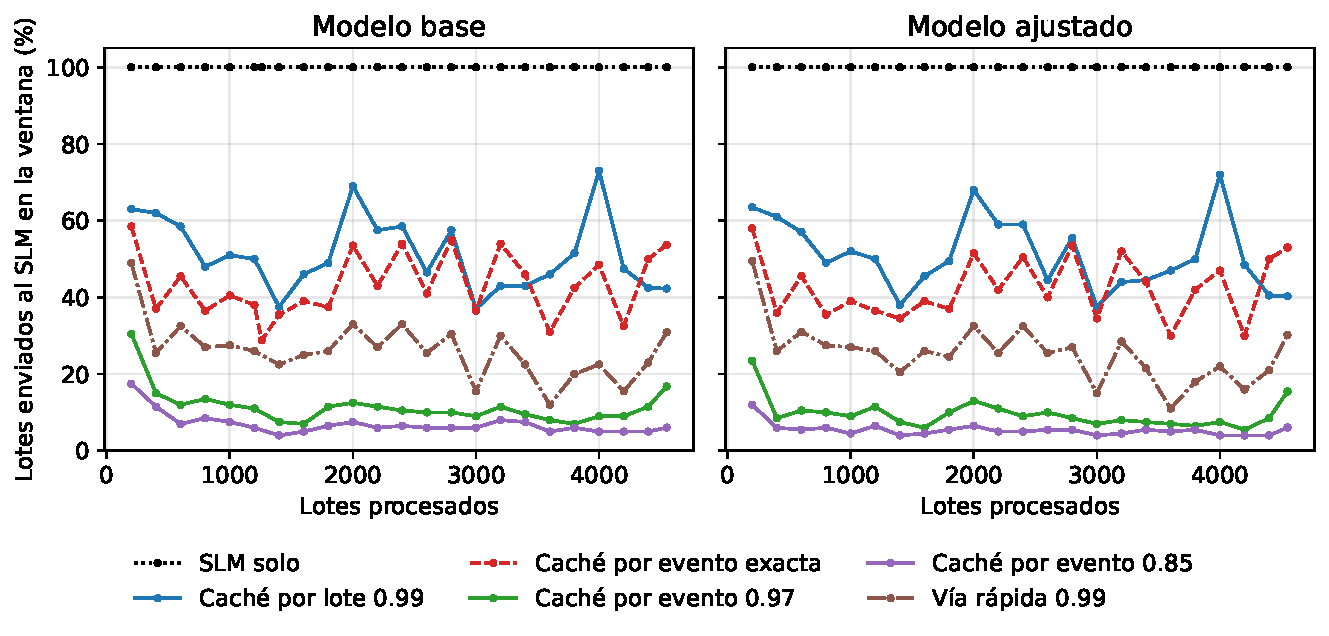
\includegraphics[width=\textwidth]{figs/resultados/uso_slm_flujo.pdf}
\caption{Porcentaje de lotes enviados al SLM por ventanas de 200 lotes a lo largo del flujo, con el modelo base y con el ajustado.}
\label{fig:res_sim_crecimiento}
\end{figure}

La dependencia del SLM bajó a lo largo del flujo en todos los métodos de caché, y sobre todo en la caché por evento con similitud: con el umbral de 0.97 y el modelo ajustado, pasó del 24\,\% de los lotes en la primera ventana al 8\,\% en los últimos 949 lotes. La caché por lote y la caché por evento exacta oscilan entre ventanas, mientras que la caché por evento con umbral bajo se mantiene estable desde las primeras ventanas. Con el modelo ajustado, la caché por evento arrancó más baja que con el base, porque marca menos lotes como error y deja, por tanto, menos eventos sospechosos. Al terminar el flujo, la caché con más vectores guardaba 5\,977, que ocupan unos 12~MB.

La detección también se comparó entre la primera y la segunda aparición del mismo lote de error. Con el SLM solo y con la caché por evento fue la misma en ambas apariciones (95.4\,\% y 94.2\,\% con el base, 93.1\,\% y 93.0\,\% con el ajustado), porque la caché por evento nunca emite una alerta por sí sola y la segunda aparición vuelve a pasar por el SLM. Con la vía rápida, entre 80 y 81 de las 86 segundas apariciones se alertaron desde la caché, y con la caché por lote de 0.97 a 0.99, entre 69 y 79 se resolvieron reutilizando la respuesta de la primera.

\subsection{Latencia de detección}

La latencia se midió de extremo a extremo en el modo de ritmo fijo, a 20 eventos por segundo, con el modelo base en el equipo 2 y 59 incidentes, como se muestra en la tabla~\ref{tab:res_sim_latencia}. El envío de la alerta tardó menos de 1~ms en ambos casos.

\begin{table}[H]
\centering
\caption{Latencia medida a 20 eventos por segundo, modelo base (1\,259 lotes, 59 incidentes). Latencia y partes en segundos.}
\label{tab:res_sim_latencia}
\footnotesize
\setlength{\tabcolsep}{4pt}
\resizebox{\textwidth}{!}{\begin{tabular}{@{}lrrrrcc@{}}
\toprule
\textbf{Método} & \textbf{Detectados} & \textbf{FA} & \textbf{MCC} & \textbf{Al SLM} & \textbf{Latencia mediana / p95 / máx.} & \textbf{Llenado / cola / análisis} \\
\midrule
SLM solo & 55 (93.2\,\%) & 117 & 0.51 & 100\,\% & 1\,777 / 3\,210 / 3\,355 & 2.5 / 1\,768 / 7.5 \\
Caché por evento exacta & 55 (93.2\,\%) & 66 & 0.63 & 42.0\,\% & 30.6 / 108.8 / 137.8 & 2.5 / 20.5 / 7.5 \\
\bottomrule
\end{tabular}}
\normalsize
\end{table}

La diferencia entre ambos métodos está en la cola. En el equipo 2, el modelo base tardó unos 5.5~segundos por lote, lo que equivale a una capacidad de unos 9 eventos por segundo, menor que el ritmo de llegada. Con el SLM solo, la cola creció durante toda la ejecución, y la mediana de la latencia llegó a unos 30 minutos. Con la caché por evento exacta, menos de la mitad de los lotes fue al SLM, de modo que la cola se mantuvo corta y la latencia mediana fue 58 veces menor, con la misma detección y menos falsas alarmas.

Estas mediciones sirvieron para validar el modelo de colas. Con el SLM solo, el modelo predijo una latencia mediana de 1\,848~segundos frente a los 1\,777 medidos, un error del 3.8\,\%. Con la caché por evento exacta predijo 68.8~segundos frente a 30.6, porque a ese ritmo el equipo trabajaba al 91\,\% de su capacidad, y cerca de la saturación la cola es muy sensible a pequeñas diferencias en los tiempos de proceso. En la tabla~\ref{tab:res_sim_colas} se presenta la latencia calculada para los demás ritmos y métodos.

\begin{table}[H]
\centering
\caption{Latencia mediana calculada con el modelo de colas, en segundos (base / ajustado). Inest.: la cola crece sin límite, porque el tiempo medio de proceso supera el intervalo entre lotes.}
\label{tab:res_sim_colas}
\footnotesize
\setlength{\tabcolsep}{4pt}
\begin{tabular}{@{}lccccc@{}}
\toprule
\textbf{Método} & \textbf{0.2 ev/s (real)} & \textbf{5 ev/s} & \textbf{10 ev/s} & \textbf{20 ev/s} & \textbf{30 ev/s} \\
\midrule
SLM solo & 253 / 248 & 17.5 / 12.8 & inest. / 7.9 & inest. / inest. & inest. / inest. \\
Caché por lote 0.98 & 252 / 248 & 16.5 / 12.7 & 11.6 / 7.8 & 10.2 / 5.4 & 98 / 4.7 \\
Caché por lote 0.99 & 252 / 248 & 17.1 / 12.8 & 12.5 / 7.9 & inest. / 5.7 & inest. / 32 \\
Caché por lote 0.995 & 253 / 248 & 17.4 / 13.1 & 19.9 / 8.2 & inest. / inest. & inest. / inest. \\
Caché por evento exacta & 253 / 248 & 17.5 / 12.8 & 12.8 / 7.9 & inest. / 5.6 & inest. / 5.6 \\
Caché por evento 0.99 & 253 / 249 & 17.6 / 13.3 & 12.8 / 8.4 & 15.5 / 6.0 & inest. / 5.4 \\
Caché por evento 0.97 & 253 / 248 & 17.6 / 13.0 & 12.7 / 8.1 & 10.3 / 5.6 & 9.7 / 4.8 \\
Caché por evento 0.85 & 253 / 248 & 17.6 / 12.9 & 12.7 / 8.0 & 10.2 / 5.5 & 9.5 / 4.7 \\
Vía rápida exacta & 245 / 245 & 9.8 / 9.8 & 7.0 / 4.9 & 37 / 3.2 & inest. / 4.6 \\
Vía rápida 0.995 & 245 / 246 & 10.0 / 10.7 & 6.7 / 5.8 & 19 / 4.8 & inest. / 5.4 \\
Vía rápida 0.99 & 245 / 246 & 9.9 / 10.5 & 5.0 / 5.6 & 8.1 / 3.2 & 86 / 4.0 \\
\bottomrule
\end{tabular}
\normalsize
\end{table}

La tabla muestra dos situaciones. Al ritmo real del servicio, la latencia es casi igual con cualquier método, porque está dominada por el llenado del lote: el incidente ocupa el lote completo, y la alerta solo puede llegar después de sus 50 eventos. La vía rápida gana unos segundos porque alerta en cuanto se cierra el lote, sin esperar al modelo. A ritmos mayores, la diferencia la marca la capacidad del SLM: el ajustado, con 2.7~segundos por lote en el equipo 1, soporta hasta unos 18 eventos por segundo, y el base en el equipo 2, con 5.5~segundos, hasta unos 9; por encima de esos ritmos, la cola crece sin límite. Con la caché por evento con similitud, ambos modelos se mantuvieron estables hasta 30 eventos por segundo, el ajustado con los umbrales de 0.85 a 0.99 y el base con los de 0.85 a 0.97, mientras que las cachés que más llaman al SLM se saturaron igual que el SLM solo.


\figpendiente{fig:res_sim_latencia}{Latencia mediana en función del ritmo de llegada de eventos.}{Eje horizontal, eventos por segundo (0.2, 5, 10, 20, 30, escala logarítmica); eje vertical, latencia mediana en segundos (escala logarítmica); una línea por método, marcando con un símbolo los ritmos inestables; un panel por modelo. Ya existen versiones en \texttt{report/latency\_vs\_rate\_\_qwen35.png} y \texttt{\_\_qwen35\_logft.png}.}

\section{Notificación y recomendación}\label{sec:res_reaccion}

La calidad de las recomendaciones no se evaluó de forma cuantitativa, y en la simulación las alertas se registraron en un archivo, sin enviarse a Slack. En la figura~\ref{fig:res_recomendacion} se muestra un ejemplo de una alerta y de la recomendación generada para un lote con error del \textit{ground truth}. El modelo ajustado escribió una descripción del error en todas sus alertas, pero dejó de proponer una acción, porque ese campo iba vacío en los ejemplos de entrenamiento; la causa probable y la acción sugerida siguen a cargo del recomendador.

\figpendiente{fig:res_recomendacion}{Ejemplo de alerta y recomendación para un lote con error.}{Fragmento del lote con error (eventos señalados), la alerta enviada a Slack y la tarjeta del \textit{dashboard} con la causa probable y la acción sugerida por el recomendador. Tomar un caso real de \texttt{recommendations.jsonl} \falta{elegir un lote con error del \textit{ground truth} con recomendación registrada}.}
